\chapter{Introduction} \label{ch:introduction}
Quadrotor control is a difficult and interesting problem. A quadrotor has six degrees of freedom (three translational and three rotational) and four independent inputs (forces applied by the motors). As established by \cite{Liu2015} and \cite{Lopez2015}, quadrotor dynamics are affected by nonlinearity, parameters perturbations, uncertainties and disturbances: this include unknown and variable payloads, aerodynamical parameters of the system, wind changes, and sensors inaccuracies. Numerous studies have been developed in designing optimal and robust controllers that allow unmanned aircraft systems (UAS) to fly and accomplish missions rejecting disturbances and being robust to parameter uncertainties as seen in \cite{Jung2014, Kohno2014, Shang2016, Salazar2014}.\\\\
Although there are embedded systems with high computational capacity that can serve as controllers of a quadrotor, smartphones are available, easily accessible for people and also have a large computational capacity, hence multiple instrumentation and communication elements integrated in the same device. The use of smartphones also facilitates distribution and installation of updates of the control application as it is a commonly known device and has application distribution platforms. Some attempts to joint smartphones and aerial robots have been made: in \cite{Pearce2014a}, a smartphone was used as a mission planner for a quadrotor and in \cite{ALEMARK2014a}, a smartphone was used as flight controller using its sensors and power to stabilize the quadrotor and control its altitude. A smartphone has been used as a flight controller and processing system for image-based positioning in a quadrotor, as shown in \cite{Loianno2015}.
\\\\
This research project aims to design and implement algorithms that will be executed in a smartphone to estimate and control quadrotor dynamics by the Research Group in Industrial Control. This project confronts several challenges such as using a smartphone as a hardware development platform, trying to use a non real-time operating system for real-time applications, designing optimal and high order controllers using Java or C++, and executing that controllers in a smartphone.
\\\\
This paper presents the design of an optimal and a robust controller, and a state estimator based on a Kalman filter for a smartphone-based quadrotor. The non-linear and linerized model of the quadrotor is presented, the controller that allows the quadrotor to follow a trajectory reference using two approachs is designed. The two approaches are the LQG and $H_\infty$ controllers. The quadrotor flight dynamics estimation strategies using sensor fusion algorithms are described. 
\\\\
In recent years, the interest in aerial robotics research has increased substantially. This is because this type of robotics offers several potential new services such as search and rescue, observation, mapping, inspection, etc. On the other hand, smartphones have become essential devices for humans and easily acquirable development tools. The interaction between these two technologies allow the development of low cost quadcopters based on an everyday item such as the smartphones, facilitating the distribution of the quadcopter control software and its implementation by other researchers.
%~\ref{fig:quads500} for an example.
\begin{figure}[h]
\begin{center}
\includegraphics[width=8.6cm]{quadBasic1}    
\caption{Assembled quadcopter used in this research with the on-board smartphone on the top center of it.} 
\label{fig:quads500}
\end{center}
\end{figure}
\\\\

In this paper, the implementation of a quadcopter with a smartphone acting as its flight controller while using exclusively the sensors and processor in the smartphone, is shown. The controller keeps the attitude of the quadcopter stabilized while making the quadcopter to hover at an altitude reference. It is presented the detailed composition of the test platform (quadcopter) used, integrating it with its dynamic model in addition to the quadcopter altitude and attitude estimation strategies using sensor fusion algorithms.
\section{Motivation}
wfwfew
\section{Research Problem}
En los últimos años el interés por la investigación en robótica aérea ha aumentado sustancialmente. Esto se debe a que este tipo de robótica ofrece diferentes servicios potenciales como búsqueda y rescate, observación, mapeo, inspección, entre otros. Por otro lado, los teléfonos inteligentes se han convertido en dispositivos esenciales para el ser humano y en herramientas de desarrollo y prototipado rápido de fácil acceso. La interacción entre estas dos tecnologías permitiría el desarrollo de cuadricópteros a bajo costo basados en un elemento cotidiano como los teléfonos inteligentes, facilitando la distribución del software de control y su implementación a manos de otros investigadores.
\\\\
Los  desafíos  de  investigación  existentes  están en  cómo  desarrollar  e  implementar  algoritmos eficientes de control para teléfonos inteligentes usando el sistema operativo Android, y  valorar,  adaptar  y  desarrollar  las  tecnologías  adecuadas  de  comunicación,  sensado  y actuación con los teléfonos inteligentes en la ejecución de misiones utilizando cuadricópteros.
\\\\
La pregunta a responder es ?`cómo desarrollar estrategias de control en un teléfono inteligente para el control de vuelo de un cuadricóptero de manera que se utilice la instrumentación y capacidad de computación del teléfono y se puedan desarrollar misiones utilizando un cuadricóptero?\\
\section{Objectives}
\subsubsection{Objetivo General}
In order to dev
Para responder a la pregunta de investigación se plantea el siguiente objetivo general:\\
Diseñar e implementar algoritmos de control y estimación de dinámicas de vuelo ejecutados en un teléfono inteligente para el cuadricóptero del Grupo de Investigación en Control Industrial.
\subsubsection{Objetivos Específicos}
\begin{enumerate}
\item Realizar un estudio y análisis del estado del arte relacionado con el control y la estimación de los estados de cuadricópteros.
\item Integrar el cuadricóptero existente con un telefono intelingente que contenga los sensores adecuados para el control y la estimación de estados.
\item Obtener un modelo dinámico del cuadricóptero.
\item Diseñar e implementar los algoritmos de control y de estimación de estados para el cuadricóptero.
\item Integrar la plataforma de experimentación con los algoritmos de control y estimación en el teléfono inteligente.
\item Evaluar el desempeño de las estrategias de control.%????
\end{enumerate}

\section{Literature Review}
wfwfewf

\subsection{Quadrotors}
wfwefwe


\subsection{Quadrotor Flight Modes}
%\url{http://ardupilot.org/copter/docs/flight-modes.html}
In quadrotors, the on-board flight controllers keep some of the quadrotors $DoF$ in a desired value autonomously in order to allow pilots to perform tasks during a flight. This controllers have different modes that can control from $3$ to $6$ $DoF$ depending on the will of the pilot. Flight modes commonly found in commercial flight controllers may be as basic to only control its attitude or as complex to let the quadrotor follow a complex trajectory with multiple waypoints \cite{Ardupilot2016}.
\\\\
The main flight modes, widely used in commercial flight controllers, are described bellow according to the number of controlled $DoF$, in ascending order.

\begin{itemize}
\item \textbf{Stabilize Mode}\\\\
This mode allows the pilot to fly the quadrotor manually while the flight controller self-levels the quadrotor attitude and regulate its current heading. Thus, the stabilize mode attempts to control three $DoF$ of the quadrotor.\\\\
The attitude references can be set or changed by the pilot using the remote control, but their default value is $0\ rad$. On the other hand, the quadrotor heading is simply set to be regulated in its current state, enabling its rate using the remote control.
\\\\
As the stabilize mode do not take into account the control of the quadrotor position, the pilot needs to regularly change the attitude references manually to keep the quadrotor in a desired position, as it is affected by wind disturbances. Also, the pilot needs to regularly adjust the quadrotor thrust, so that a desired altitude is maintained.

\item \textbf{Altitude Hold Mode}\\\\
The altitude hold mode adds automatic elevation control to the Stabilize mode. This way, in addition to controlling the attitude, the quadrotor thrust is set by the flight controller in order to maintain the quadrotor in a desired altitude, getting four controlled $DoF$.
\\\\
In this mode, the pilot can remotely control the rate of change of the elevation (with a default value of $0\ m/s$), as well as the attitude references.

\item \textbf{Loiter Mode}\\\\
Loiter mode automatically attempts to regulate the six $DoF$ of the quadrotor in order to maintain a desired position, heading and altitude during a flight. Here, the quadrotor attitude is self-leveled, while the position and altitude reference can be modified by the pilot using the remote controller. The position and altitude references are initialized using the current quadrotor position and altitude when this mode is set. This is a GNSS-Dependent flight mode.

\item \textbf{Auto Mode}\\\\
The Auto mode attempts to make a quadrotor follow automatically a pre-programmed path connecting multiple position and heading waypoints, while receiving . This mode use the same controller as the Loiter mode, but its references are set automatically following the waypoints list. As in Auto mode the quadrotor must follow geo-located waypoints, this is a GNSS-Dependent flight mode.

\item \textbf{Return-To-Launch Mode}\\\\
During a flight mission, the home location is set as the position and altitude where the quadrotor took off. The Return-To-Launch mode is used in case of emergency or when a the last waypoint is reached within a flight mission. This mode is equivalent to the Auto mode, but only has two waypoints. The first waypoint consists in the position of the home location with a previously set altitude ($RTL$ altitude) greater than the home altitude. When this waypoint is reached, the home location is set as the following waypoint so that the quadrotor starts its landing keeping the position controlled.

\end{itemize}


\subsection{Smartphones as Controllers}
Current smartphone processors are able to perform complex calculations such as those required in the implementation of real time control strategies. There are many ongoing research related to the possibility of using smartphones to implement control strategies, such as \cite{Drumea2013a}, as configuration and monitoring interfaces in control systems as seen in \cite{Lin2014a,Truong2012a}, and as a tool in both education and design of control strategies seen in \cite{Aristizabal2014a,WuWu2013a}. Following this trend, in the Universidad del Valle, it was developed a smartphone-based platform for monitoring, control and communication in portable laboratories, where a controller for a pendulum based in the Lego Mindstorms EV3 platform was implemented \cite {GarciaTellez2015}.
\\\\

\subsection{Smartphone-based Quadrotors}
In the University of Pennsylvania, in \cite{Loianno2015}, was developed a quadcopter using a last generation smartphone as a flight controller and an additional processing system for image-based positioning. The state estimation algorithms, control and planning were firstly implemented in a ODROID-XU board with additional sensors, but then, in \cite{Loianno2015a}, this algorithms were ported to the Qualcomm processor in the phone due to the Qualcomm colaboration in that project.
\\\\
Current research focuses on the development of aerial robots potentiated by the use of smartphones, as seen in \cite{Pearce2014a, ALEMARK2014a, Aldrovandi2015, Bryant2015}. In the last years, computing capacity and sensor technology in smartphones has decreased in price but increased in performance. Smartphones have become an inexpensive tool capable of commanding an UAV. The challenge then, is to use smartphones as quadcopter flight controllers for autonomous flights following specific missions, taking advantage of the fact that the phones today are very powerful computers that include elements of sensing, processing and signal communication.
\\\\

\subsubsection{Smartphone-based Quadrotor Limitations}
The idea of using a smartphone as flight controller in an UAV opens the possibility of a rapid and inexpensive development \cite{Aldrovandi2015}. A smartphone offers other advantages compared with off-the-shelf flight controllers, for instance its powerful quad or hexa-core processors and communications interfaces. However, smartphones and the Android operating system have some limitations that set challenges when implementing a control system in it.\\\\
Android is not a real-time operating system and thus can not assure execution of algorithms, like estimation and control, with a constant sample time. Furthermore, the sensors embedded in commercial smartphones are made for applications that do not have high requirements of accuracy nor precision and therefore may not be appropriate for sensing quadrotor dynamics. Nonetheless, as explained by \cite{Bryant2015}, due to its computing capabilities, smartphones can overcome this limitations while using a temporized thread to execute the control system algorithms and implement a sensor fusion technique to improve the states estimation reliability. This thread must be executed with a lower sample time compared to the one of the sensors embedded in the smartphone. This will ensure that the execution is not delayed by the sensors acquisition process.

\section{Outline}
In the next section, a detailed description of the hardware used in the quadcopter is presented. After that, the dynamic non-linear and linearized quadcopter model is shown in Section \ref{sec:Model}. In Section \ref{sec:Controller}, all the aspects related to the altitude and attitude cascade controllers design are presented.
Then, in Section \ref{sec:Estimation} the sensor fusion algorithm that is used to estimate the altitude of the quadcopter, and how the orientation of the system is estimated, is described. In Section \ref{sec:Implementation}, the implementation in Android of all the necessary software with its results is provided. Finally, Section \ref{sec:Conclusion} concludes this paper taking into account the results of this research and the future work to be done.
\\\\
This paper is organized as follows: The smartphone-based quadrotors features and limitations are shown in Section \ref{sec:limitations}. In Section \ref{sec:Model}, the dynamic model of a quadrotor in $X$-configuration using a Newton-Euler approach is presented. After that, in Section \ref{sec:controllers}, the quadrotor parameters and controllers design procedure is exposed. In Section \ref{sec:estimation}, the state estimation algorithms based on a Kalman filter and the kinematic model of a particle with constant acceleration are provided. The performance of the proposed flight control system through simulations is presented in Section \ref{sec:simulation}. Finally, Section \ref{sec:conclusions} shows the conclusions and future aiming of this project.

%\section{Multi-Agent Systems}
%
%
%Advances in exploration and rescue technologies become more relevant than ever before.
%
%In an effort to develop distributed mobile agent systems able to resemble their natural counterparts, engineers have been experimenting with mobile sensor networks trying, for example, to implement flocking applications.  The goal has been to create self-organized networks  capable of coordinated group behaviour \citep{MateiBaras12}. For this purpose, heuristic rules were introduced by \citep{SpanosOlfatiMurray05} in order to explain any form of collective behaviour of a large number of individuals  with a common goal. These rules are known as cohesion, separation, and alignment. Cohesion means the attempt to stay close to  the neighbours, separation means avoiding collisions with neighbours, and alignment means the attempt to match velocity with neighbour agents. 
%
%
% For example, oil spilled in the sea generates a scalar field of oil concentration values (Fig. \ref{fig:oilspill}). Similarly,  radiation levels after  nuclear disaster like in Fukushima (Fig.  \ref{fig:fukushima_1}), or a toxic substance cloud moving in space are  phenomena that can be represented as scalar fields (Fig. \ref{fig:scalarfieldsource}). 
%\afterpage{
%\begin{figure}[ht!]
%        \centering
%        \begin{subfigure}[t]{0.49\textwidth}
%                \includegraphics[width=\textwidth]{oilspill.eps}
%                \caption{Oil spill \footnotemark} 
%                \label{fig:oilspill}
%        \end{subfigure}%
%        ~ %add desired spacing between images, e. g. ~, \quad, \qquad etc.
%          %(or a blank line to force the subfigure onto a new line)
%        \begin{subfigure}[t]{0.49\textwidth}
%                \includegraphics[width=\textwidth]{fukushima_1.eps}
%                \caption{Fukushima's environment radiation levels after nuclear disaster  \footnotemark}
%                \label{fig:fukushima_1}
%        \end{subfigure}
%        ~ %add desired spacing between images, e. g. ~, \quad, \qquad etc.
%          %(or a blank line to force the subfigure onto a new line)
%        \begin{subfigure}[t]{0.62\textwidth}
%                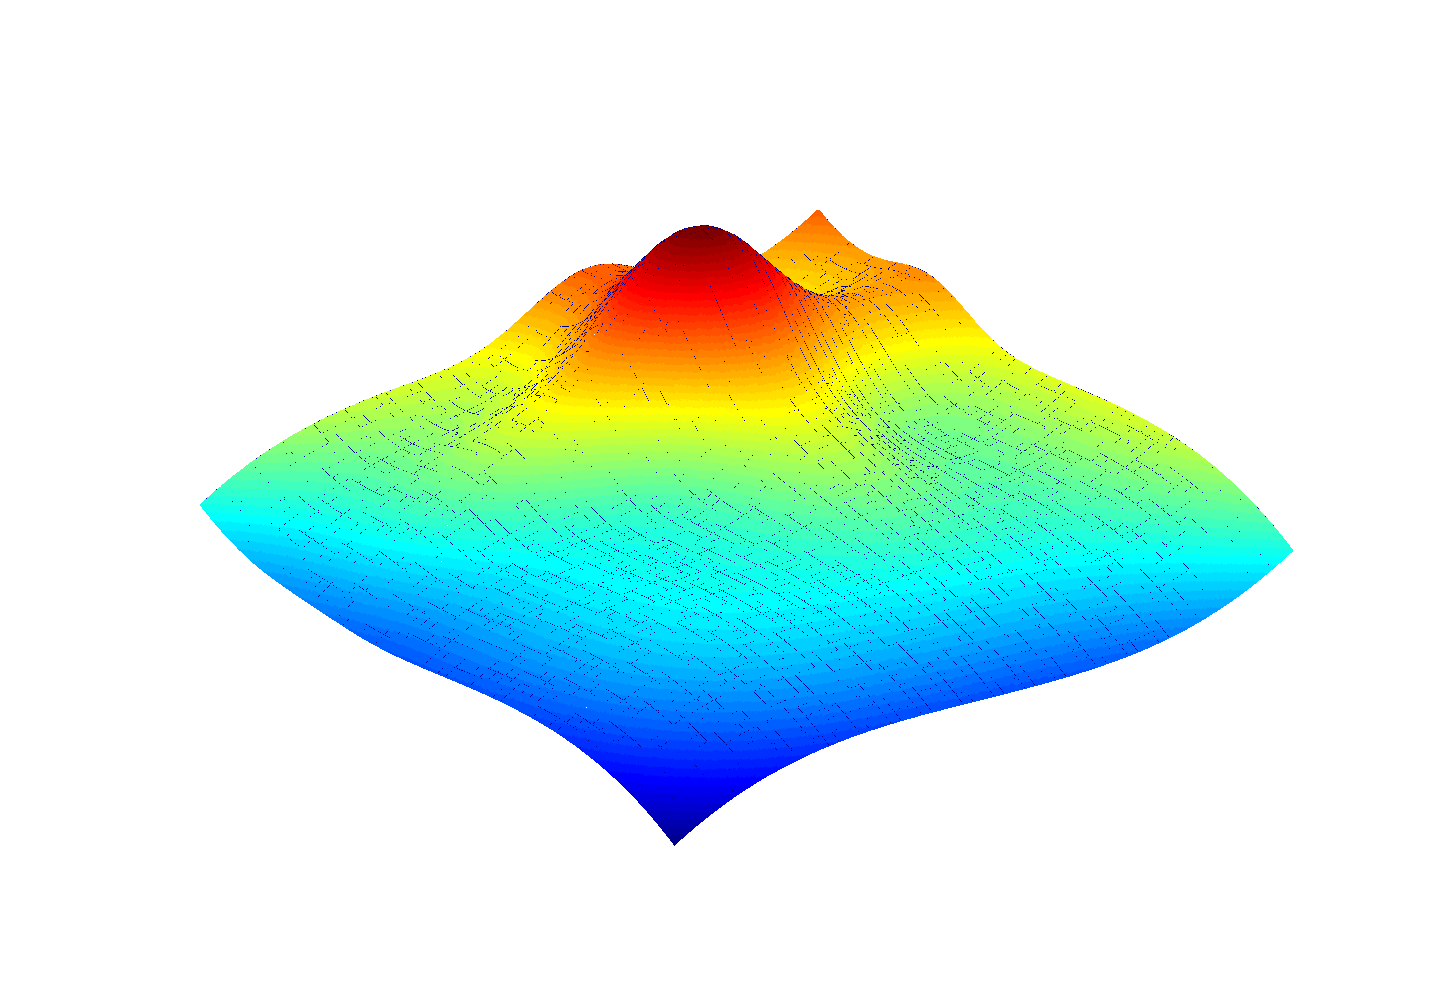
\includegraphics[width=\textwidth]{scalarfieldsource.eps}
%                \caption{Toxic cloud}
%                \label{fig:scalarfieldsource}
%        \end{subfigure}%
%        ~ %add desired spacing between images, e. g. ~, \quad, \qquad etc.
%          %(or a blank line to force the subfigure onto a new line)
%       \caption{Scalar fields} \label{fig:scalar field}
%\end{figure}
%\footnotetext[1]{Picture taken from FeedNetBack project}
%\footnotetext[2]{Picture taken from seaandskyjp.wordpress.com}
%}
% 


